% Provenance (never printed): cycle 4 SVT, "La planete Terre": volcanic
% activity, its products and its link with plate boundaries; natural hazards
% and their monitoring; see sources/book1/PROVENANCE.md. Book 1, grade 7,
% chapter 2.
% Vocabulary guard: "magma" first allowed here; "sediment" not before g7.4;
% "subduction zone" is never a term here (gloss: "where one plate sinks under
% another"); "hotspot track" is Book 2's; lahars are called mudflows.
\chapter{Gunung Api}\label{ch:g7:volcanoes}

Pada tanggal 17~Mei 1980, seorang ahli geologi berdiri di sebuah punggung
\omterm{def:g1:landscapes-around-us:landform}{bukit} sepuluh kilometer dari Gunung St.~Helens, di barat laut Amerika
Serikat, dan mengambil foto di sebelah kiri bawah ini: kerucut yang mulus
dan bersalju, salah satu \omterm{def:g1:landscapes-around-us:landform}{gunung} paling anggun di negeri itu. Selama dua
bulan \omterm{def:g1:landscapes-around-us:landform}{gunung} itu terus bergetar, dan lereng utaranya menggembung ke luar
seperti balon. Keesokan paginya, pukul 08.32, sebuah \omterm{def:g4:volcanoes-earthquakes-first-look:earthquake}{gempa bumi} kecil
mengguncangnya. Seluruh lereng yang menggembung itu longsor, dan \omterm{def:g4:volcanoes-earthquakes-first-look:volcano}{gunung api}
itu meletus ke samping. Ketika punggung \omterm{def:g1:landscapes-around-us:landform}{bukit} yang sama dapat difoto lagi,
pada bulan September, \omterm{def:g1:landscapes-around-us:landform}{gunung} itu tampak seperti foto di sebelah kanan.

\begin{omfigure}
\begin{minipage}[b]{0.495\linewidth}\centering
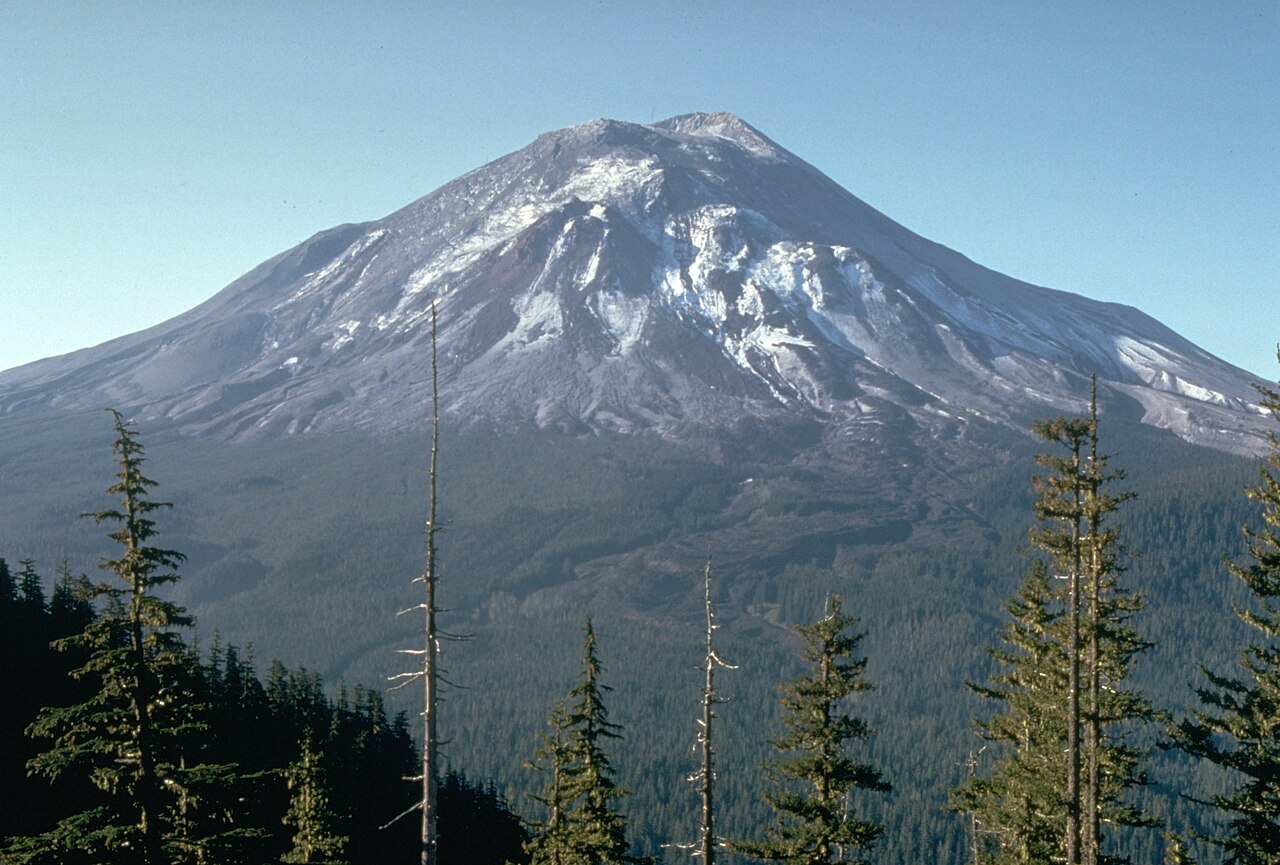
\includegraphics[width=\linewidth]{images/book1/g7-msh-before.jpg}

{\small 17 Mei 1980, sehari sebelumnya.}
\end{minipage}\hfill
\begin{minipage}[b]{0.495\linewidth}\centering
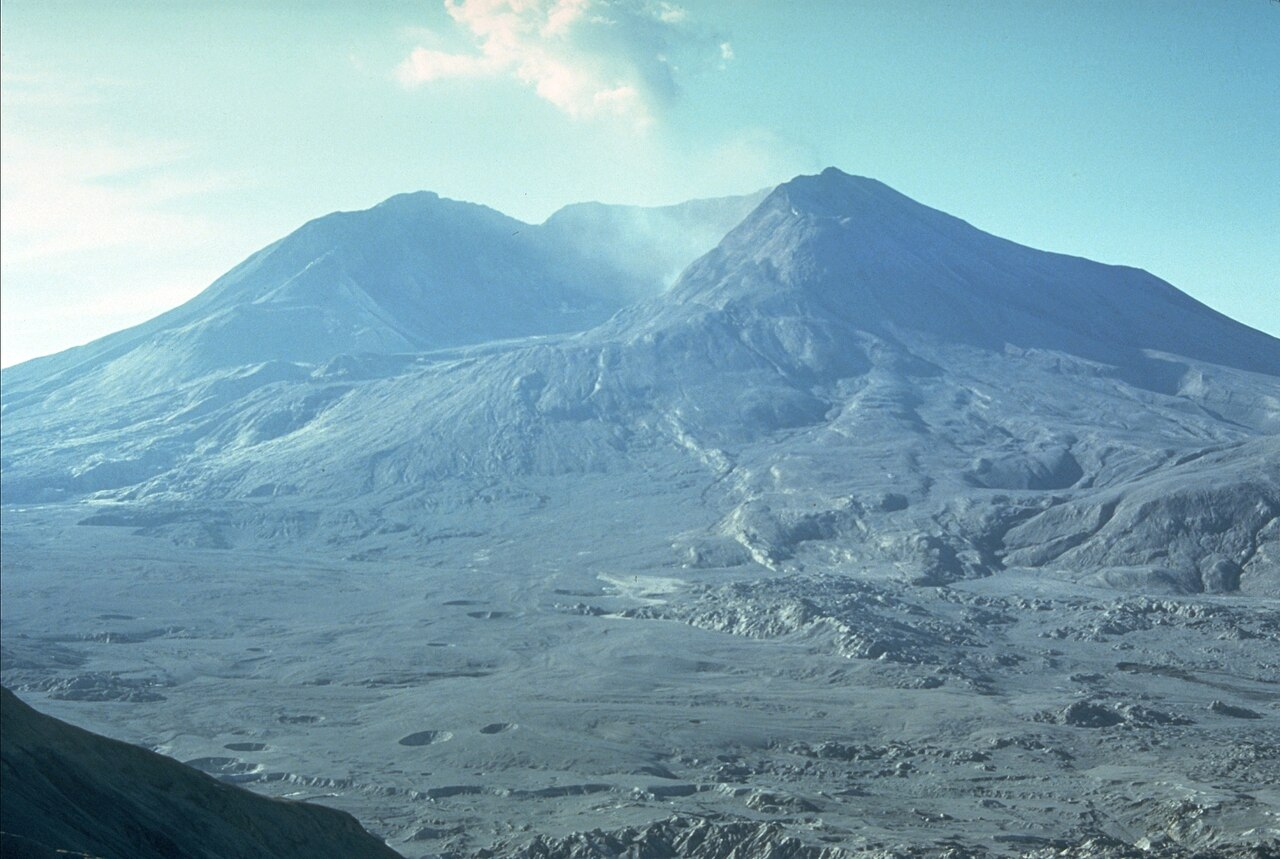
\includegraphics[width=\linewidth]{images/book1/g7-msh-after.jpg}

{\small 10 September 1980.}
\end{minipage}

{\small Gunung St.~Helens dilihat dari Johnston Ridge, sebelum dan sesudah
\omterm{def:g4:volcanoes-earthquakes-first-look:eruption}{letusan} tanggal 18~Mei 1980. Puncaknya dan seluruh lereng utaranya hilang;
sebuah \omterm{def:g7:volcanoes:vent}{kawah} yang terbuka ke arah utara menggantikannya. Foto: Harry
Glicken, U.S. Geological Survey (domain publik, melalui Wikimedia Commons).}
% ledger: commons:msh-before, commons:msh-after, usgs:msh-lead-up, usgs:msh-may18
\label{fig:g7:volcanoes:st-helens}
\end{omfigure}

Dalam bab ini kita membuka sebuah \omterm{def:g4:volcanoes-earthquakes-first-look:volcano}{gunung api}, untuk melihat apa yang
mendorong \omterm{def:g4:volcanoes-earthquakes-first-look:eruption}{letusan}; kita mencari tahu mengapa sebagian \omterm{def:g4:volcanoes-earthquakes-first-look:volcano}{gunung api}
mengalirkan \omterm{def:g1:landscapes-around-us:water}{sungai} \omterm{def:g4:volcanoes-earthquakes-first-look:eruption}{lava} yang tenang, sedangkan yang lain meledakkan dirinya
sendiri; dan kita melihat lagi \omterm{def:g3:continents-and-oceans:world-map}{peta dunia}, untuk mengetahui di mana letak
\omterm{def:g4:volcanoes-earthquakes-first-look:volcano}{gunung-gunung api} dan mengapa.

\begin{recall}
Yang disebut \emph{\omterm{def:g4:volcanoes-earthquakes-first-look:volcano}{gunung api}} adalah tempat \omterm{def:g3:stones-pebbles-sand:rock}{batuan} cair dari dalam Bumi
keluar ke permukaan, dan juga \omterm{def:g1:landscapes-around-us:landform}{bukit} atau \omterm{def:g1:landscapes-around-us:landform}{gunung} yang dibangunnya di sana.
Ketika \emph{\omterm{def:g4:volcanoes-earthquakes-first-look:eruption}{letusan}}, \omterm{def:g4:volcanoes-earthquakes-first-look:volcano}{gunung api} memuntahkan \omterm{def:g4:volcanoes-earthquakes-first-look:eruption}{lava}, abu, dan gas
(\cref{ch:g4:volcanoes-earthquakes-first-look}). Di bawah \omterm{def:g6:inside-the-earth:layers}{kerak}, \omterm{def:g6:inside-the-earth:layers}{mantel}
terdiri atas \omterm{def:g3:stones-pebbles-sand:rock}{batuan} panas yang padat, walaupun \omterm{def:g3:stones-pebbles-sand:rock}{batuan} itu dapat merayap
dengan sangat lambat (\cref{ch:g6:inside-the-earth}). Basal dan granit
adalah \omterm{def:g6:rocks-and-minerals:rock-families}{batuan beku}: \omterm{def:g3:stones-pebbles-sand:rock}{batuan} ini terbentuk ketika \omterm{def:g3:stones-pebbles-sand:rock}{batuan} cair mendingin dan
mengeras (\cref{ch:g6:rocks-and-minerals}). Cangkang luar Bumi terpecah
menjadi \omterm{def:g7:plate-tectonics:plate}{lempeng-lempeng} yang bergerak beberapa sentimeter setahun; tepinya
adalah \omterm{def:g7:plate-tectonics:plate-boundary}{batas lempeng} (\cref{ch:g7:plate-tectonics}).
\end{recall}

\section{Di dalam gunung api}

\omterm{def:g6:inside-the-earth:layers}{Mantel} itu padat. Namun di beberapa tempat, jauh di bawah permukaan,
sebagian kecil \omterm{def:g3:stones-pebbles-sand:rock}{batuannya} meleleh. \omterm{def:g3:stones-pebbles-sand:rock}{Batuan} cair itu lebih ringan daripada
\omterm{def:g3:stones-pebbles-sand:rock}{batuan} padat di sekelilingnya, sehingga \omterm{def:g3:stones-pebbles-sand:rock}{batuan} cair itu naik perlahan,
menyusup melalui retakan-retakan, seperti setetes minyak yang naik di dalam
air.
% ledger: usgs:hawaii-hotspot (magma lighter than the surrounding rock, rises)

\begin{definition}[Magma]\label{def:g7:volcanoes:magma}
Yang disebut \emph{magma}\index{magma} adalah \omterm{def:g3:stones-pebbles-sand:rock}{batuan} cair di bawah tanah.
Magma adalah cairan panas yang dapat juga membawa kristal dan, terlarut di
dalamnya, gas-gas seperti uap air dan karbon dioksida. Magma yang keluar
ke permukaan disebut \omterm{def:g4:volcanoes-earthquakes-first-look:eruption}{lava}; ketika keluar, \omterm{def:g4:volcanoes-earthquakes-first-look:eruption}{lava} kehilangan sebagian besar
gasnya.
\end{definition}

\omterm{def:g7:volcanoes:magma}{Magma} yang naik sering berhenti di tengah jalan, beberapa kilometer di
bawah permukaan, dan berkumpul di sebuah kantong besar. Di sana \omterm{def:g7:volcanoes:magma}{magma} itu
menunggu, kadang-kadang berabad-abad, sebelum sebuah \omterm{def:g4:volcanoes-earthquakes-first-look:eruption}{letusan} mengosongkan
sebagiannya.

\begin{definition}[Dapur magma]\label{def:g7:volcanoes:magma-chamber}
Yang disebut \emph{dapur magma}\index{dapur magma} adalah ruang besar di
dalam \omterm{def:g3:stones-pebbles-sand:rock}{batuan} di bawah \omterm{def:g4:volcanoes-earthquakes-first-look:volcano}{gunung api}, beberapa kilometer di bawah permukaan,
tempat \omterm{def:g7:volcanoes:magma}{magma} berkumpul sebelum \omterm{def:g4:volcanoes-earthquakes-first-look:eruption}{letusan}.
\end{definition}

\begin{definition}[Lubang letusan dan kawah]\label{def:g7:volcanoes:vent}
Yang disebut \emph{lubang letusan}\index{lubang letusan} adalah bukaan di
permukaan tempat \omterm{def:g7:volcanoes:magma}{magma}, gas, dan abu keluar. Yang disebut
\emph{kawah}\index{kawah} adalah cekungan berbentuk mangkuk di sekeliling
lubang \omterm{def:g4:volcanoes-earthquakes-first-look:eruption}{letusan}, biasanya di puncak \omterm{def:g4:volcanoes-earthquakes-first-look:volcano}{gunung api}.
\end{definition}

\begin{omfigure}
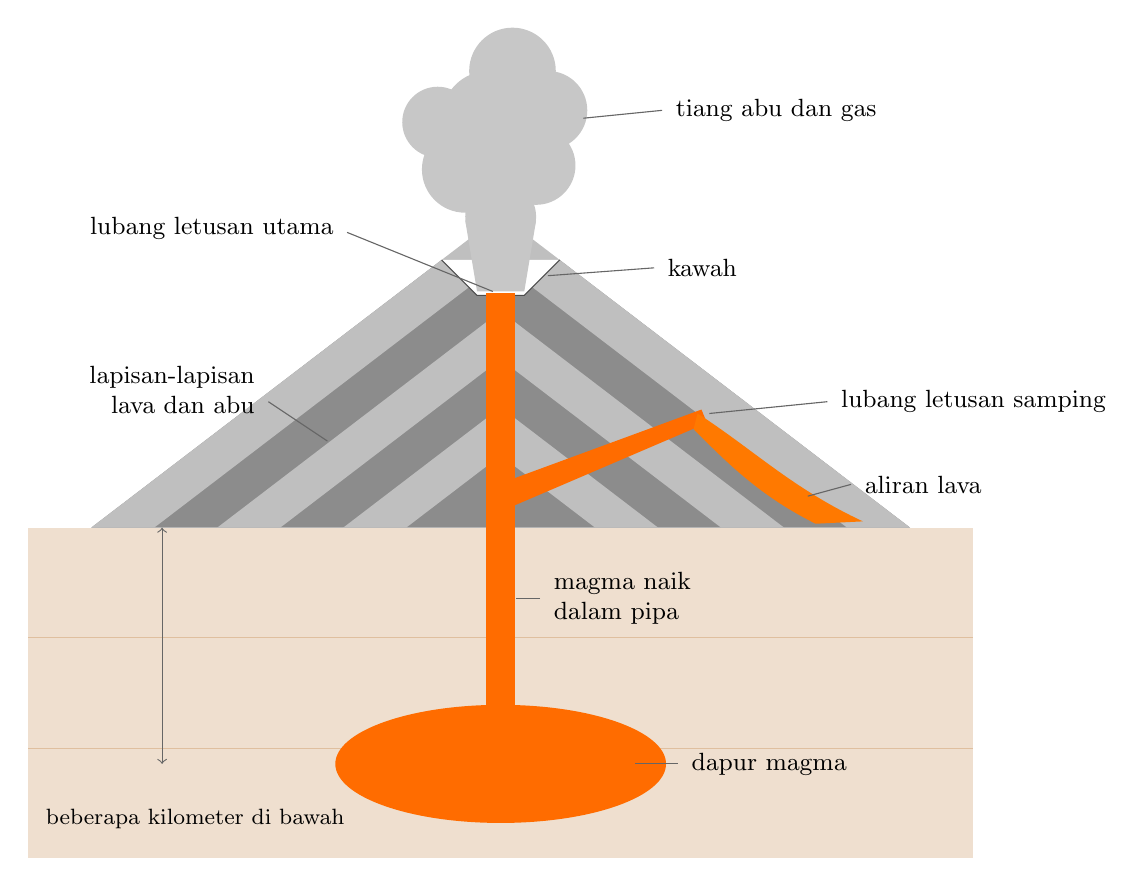
\begin{tikzpicture}[font=\small, x=1cm, y=1cm]
  % rocks below the volcano
  \fill[brown!25] (-6,-4.2) rectangle (6,0);
  \draw[brown!50] (-6,-1.4) -- (6,-1.4) (-6,-2.8) -- (6,-2.8);
  % the cone, built of layers of lava (dark) and ash (light)
  \fill[black!45] (-5.2,0) -- (-0.75,3.4) -- (0.75,3.4) -- (5.2,0) -- cycle;
    % layers dipping outwards, parallel to the flanks (slope 3.4/4.45)
  \foreach \k/\c in {0/black!25, 2/black!25, 4/black!25} {
    \pgfmathsetmacro{\xa}{-5.2+0.8*\k}\pgfmathsetmacro{\xb}{-5.2+0.8*(\k+1)}
    \pgfmathsetmacro{\ya}{(-0.18-\xa)*3.4/4.45}\pgfmathsetmacro{\yb}{(-0.18-\xb)*3.4/4.45}
    \fill[\c] (\xa,0) -- (-0.18,\ya) -- (-0.18,\yb) -- (\xb,0) -- cycle;
    \fill[\c] (-\xa,0) -- (0.18,\ya) -- (0.18,\yb) -- (-\xb,0) -- cycle;
  }
  % the crater at the top
  \fill[white] (-0.75,3.4) -- (-0.3,2.95) -- (0.3,2.95) -- (0.75,3.4) -- cycle;
  \draw[black!70] (-0.75,3.4) -- (-0.3,2.95) -- (0.3,2.95) -- (0.75,3.4);
  % magma chamber and the pipe up to the vent
  \fill[orange!85!red] (0,-3.0) ellipse (2.1 and 0.75);
  \fill[orange!85!red] (-0.18,-2.4) rectangle (0.18,2.98);
  % a side branch to a small side vent
  \fill[orange!85!red] (0.1,0.6) -- (2.55,1.5) -- (2.62,1.33) -- (0.1,0.25) -- cycle;
  % lava flow down the right flank, from the side vent
  \fill[orange!95!red] (2.5,1.45) .. controls (3.2,1.0) and (3.7,0.5) .. (4.6,0.08)
    -- (4.0,0.05) .. controls (3.3,0.4) and (2.9,0.8) .. (2.45,1.25) -- cycle;
  % ash column and gas
    \fill[black!22] (-0.3,3.0) -- (0.3,3.0) -- (0.45,3.9) -- (-0.45,3.9) -- cycle;
  \foreach \x/\y/\r in {0/3.95/0.45, -0.45/4.55/0.55, 0.45/4.6/0.5, -0.15/5.2/0.6,
                        0.6/5.3/0.5, -0.8/5.15/0.45, 0.15/5.8/0.55}
    \fill[black!22] (\x,\y) circle (\r);
  % labels
  \node[anchor=west] at (2.1,5.3) {tiang abu dan gas};
  \draw[black!60] (2.05,5.3) -- (1.05,5.2);
  \node[anchor=west] at (2.0,3.3) {kawah};
  \draw[black!60] (1.95,3.3) -- (0.6,3.2);
  \node[anchor=east] at (-2.0,3.8) {lubang letusan utama};
  \draw[black!60] (-1.95,3.75) -- (-0.1,3.0);
  \node[anchor=west] at (4.2,1.6) {lubang letusan samping};
  \draw[black!60] (4.15,1.6) -- (2.65,1.45);
  \node[anchor=west] at (4.5,0.55) {aliran lava};
  \draw[black!60] (4.45,0.55) -- (3.9,0.4);
  \node[anchor=east, align=right] at (-3.0,1.75) {lapisan-lapisan\\lava dan abu};
  \draw[black!60] (-2.95,1.6) -- (-2.2,1.1);
  \node[anchor=west, align=left] at (0.55,-0.9) {magma naik\\dalam pipa};
  \draw[black!60] (0.5,-0.9) -- (0.2,-0.9);
  \node[anchor=west] at (2.3,-3.0) {dapur magma};
  \draw[black!60] (2.25,-3.0) -- (1.7,-3.0);
  \node[anchor=west, align=left, font=\footnotesize] at (-5.9,-3.7) {beberapa kilometer di bawah};
  \draw[black!60, <->] (-4.3,0) -- (-4.3,-3.0);
\end{tikzpicture}

{\small \omterm{def:g4:volcanoes-earthquakes-first-look:volcano}{Gunung api} yang dibelah (gambar, tidak berskala). \omterm{def:g7:volcanoes:magma}{Magma} berkumpul
di \omterm{def:g7:volcanoes:magma-chamber}{dapur magma} lalu naik melalui sebuah pipa ke \omterm{def:g7:volcanoes:vent}{lubang letusan} utama, di
dasar \omterm{def:g7:volcanoes:vent}{kawah}; sebuah cabang mencapai \omterm{def:g7:volcanoes:vent}{lubang letusan} samping di lereng.
Setiap \omterm{def:g4:volcanoes-earthquakes-first-look:eruption}{letusan} menambahkan selapis \omterm{def:g4:volcanoes-earthquakes-first-look:eruption}{lava} atau abu pada kerucutnya.}
\label{fig:g7:volcanoes:cutaway}
\end{omfigure}

Jadi \omterm{def:g3:stones-pebbles-sand:rock}{batuan} cair yang sama mempunyai dua nama. Di bawah tanah namanya
\emph{\omterm{def:g7:volcanoes:magma}{magma}}; begitu keluar dari \omterm{def:g7:volcanoes:vent}{lubang letusan}, namanya \emph{\omterm{def:g4:volcanoes-earthquakes-first-look:eruption}{lava}}.
Perbedaannya bukan hanya soal kata: \omterm{def:g7:volcanoes:magma}{magma} masih menyimpan gasnya, sedangkan
\omterm{def:g4:volcanoes-earthquakes-first-look:eruption}{lava} sudah melepaskan sebagian besar gasnya ke udara. Kita akan melihat
bahwa gas inilah yang menentukan jenis \omterm{def:g4:volcanoes-earthquakes-first-look:eruption}{letusan} sebuah \omterm{def:g4:volcanoes-earthquakes-first-look:volcano}{gunung api}.

Seberapa panaskah \omterm{def:g4:volcanoes-earthquakes-first-look:eruption}{lava} itu? Para ilmuwan Hawaiian Volcano Observatory
mengukur \omterm{def:g4:volcanoes-earthquakes-first-look:eruption}{lava} yang keluar dari lubang-lubang \omterm{def:g4:volcanoes-earthquakes-first-look:eruption}{letusan} Kilauea, salah satu
\omterm{def:g4:volcanoes-earthquakes-first-look:volcano}{gunung api} di Hawaii: kira-kira \qty{1170}{\degreeCelsius}. \omterm{def:g3:stones-pebbles-sand:rock}{Batuan} panas
berpijar, dan warna pijarnya bergantung pada suhunya: kamera khusus dapat
membaca suhu sebuah aliran dari jauh dengan mengukur warna pijarnya. Mata
pun dapat memperkirakannya secara kasar, seperti yang ditunjukkan tabel ini.
% ledger: usgs:kilauea-temp, usgs:pyrometer

\begin{center}
\small
\begin{tabular}{|l|c|}
\hline
\textbf{warna \omterm{def:g3:stones-pebbles-sand:rock}{batuan} yang berpijar} & \textbf{suhu} \\
\hline
kuning & kira-kira 1000 sampai \qty{1200}{\degreeCelsius} \\
oranye & kira-kira 800 sampai \qty{1000}{\degreeCelsius} \\
merah & kira-kira 600 sampai \qty{800}{\degreeCelsius} \\
\hline
\end{tabular}
\end{center}
% ledger: usgs:kilauea-temp

\begin{remark}[Kulit yang mendingin dalam sedetik]\label{rem:g7:volcanoes:skin}
% ledger: usgs:kilauea-temp
Ketika \omterm{def:g4:volcanoes-earthquakes-first-look:eruption}{lava} pertama kali bertemu udara, permukaannya mendingin ratusan
derajat setiap detik: seketika terbentuk kulit gelap pada \omterm{def:g3:stones-pebbles-sand:rock}{batuan} yang
berpijar itu. Di bawah kulit itu, \omterm{def:g4:volcanoes-earthquakes-first-look:eruption}{lava} tetap panas untuk waktu yang lama.
Di Hawaii, \omterm{def:g4:volcanoes-earthquakes-first-look:eruption}{lava} pernah mengalir di dalam terowongan di bawah atapnya sendiri
yang sudah mengeras sejauh \qty{10}{km}, dari \omterm{def:g7:volcanoes:vent}{lubang letusan} sampai ke
\omterm{def:g2:water-on-earth:ocean}{laut}, dan masih mencapai pantai pada suhu kira-kira
\qty{1140}{\degreeCelsius}: hanya kira-kira 30~derajat lebih dingin daripada
di \omterm{def:g7:volcanoes:vent}{lubang letusan}.
\end{remark}

\begin{omfigure}
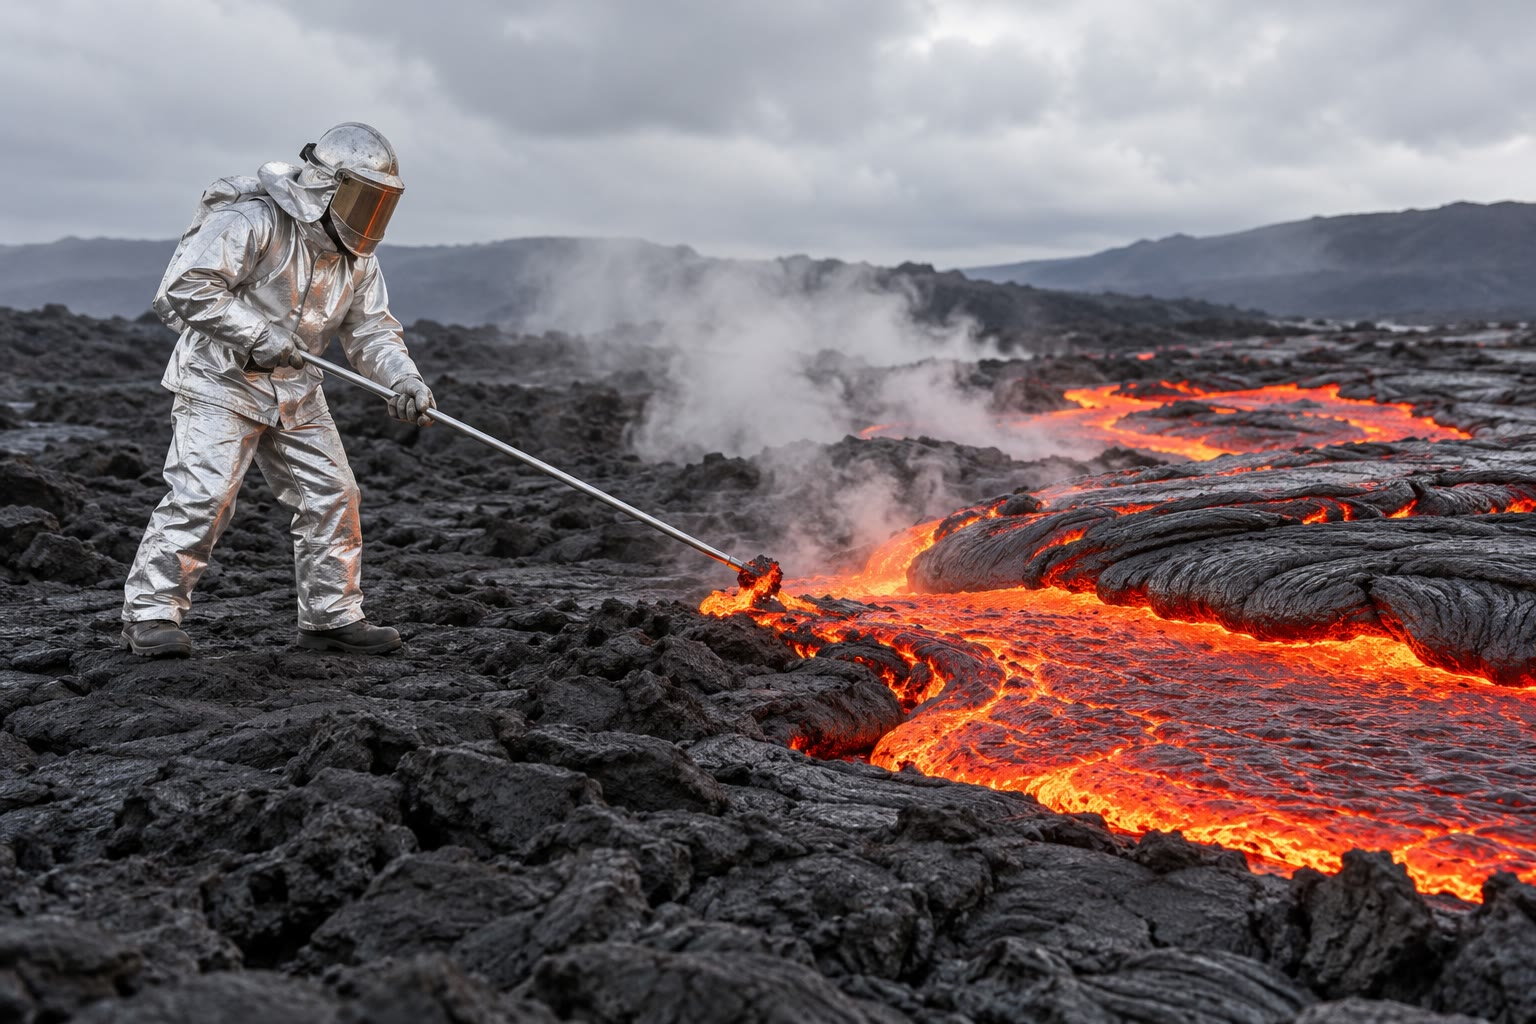
\includegraphics[width=0.6\linewidth]{images/book1/ai/g7-volcanologist.jpg}

{\small Seorang ahli \omterm{def:g4:volcanoes-earthquakes-first-look:volcano}{gunung api} yang memakai baju pemantul panas mengambil
contoh \omterm{def:g4:volcanoes-earthquakes-first-look:eruption}{lava} dengan sebatang tongkat baja yang panjang (ilustrasi AI dari
suatu adegan umum). Hanya ilmuwan terlatih, dengan perlengkapan semacam
ini, yang mendekati \omterm{def:g4:volcanoes-earthquakes-first-look:eruption}{lava} yang sedang mengalir; orang lain menonton dari
tempat yang diizinkan oleh pihak berwenang.}
\label{fig:g7:volcanoes:volcanologist}
\end{omfigure}

\section{Dua cara meletus}

Gunung St.~Helens meledakkan dirinya sendiri. Sebaliknya, \omterm{def:g4:volcanoes-earthquakes-first-look:volcano}{gunung-gunung api}
di Hawaii biasanya mengalirkan \omterm{def:g4:volcanoes-earthquakes-first-look:eruption}{lava} yang meluncur turun di lerengnya. Para
ahli geologi membagi \omterm{def:g4:volcanoes-earthquakes-first-look:eruption}{letusan} menjadi dua jenis.

\begin{definition}[Erupsi efusif dan erupsi eksplosif]\label{def:g7:volcanoes:eruption-types}
Pada \emph{erupsi efusif}\index{erupsi efusif}, \omterm{def:g7:volcanoes:magma}{magma} keluar dengan tenang
sebagai \omterm{def:g4:volcanoes-earthquakes-first-look:eruption}{lava}, yang mengalir menjauhi \omterm{def:g7:volcanoes:vent}{lubang letusan}, kadang-kadang sampai
berkilometer-kilometer, atau menyembur ke atas sebagai air mancur
tetes-tetes yang berpijar. Pada \emph{erupsi
eksplosif}\index{erupsi eksplosif}, \omterm{def:g7:volcanoes:magma}{magma} dihancurkan berkeping-keping oleh
gasnya sendiri: tiang abu, gas, dan bongkah \omterm{def:g3:stones-pebbles-sand:rock}{batuan} dilemparkan tinggi ke
langit.
\end{definition}

\begin{omfigure}
\begin{minipage}[t]{0.49\linewidth}\centering
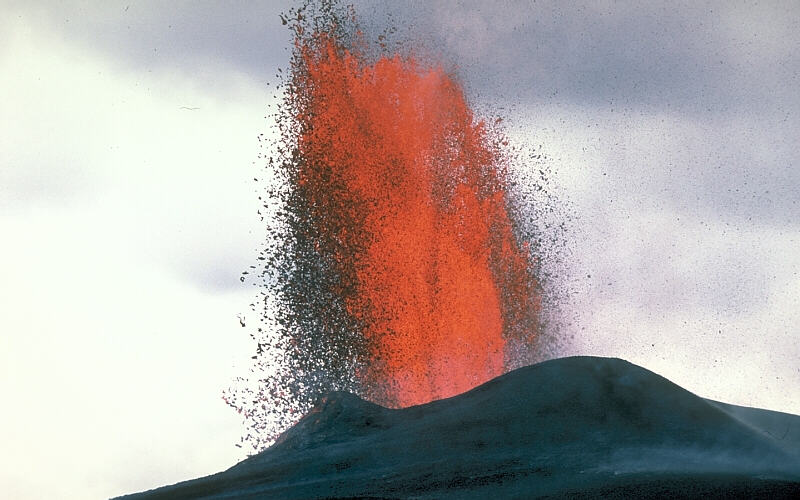
\includegraphics[height=4.5cm]{images/book1/g7-lava-fountain.jpg}

{\small Efusif: air mancur \omterm{def:g4:volcanoes-earthquakes-first-look:eruption}{lava} di Kilauea, Hawaii, 1983.
Foto: J.~D. Griggs, USGS.}
\end{minipage}\hfill
\begin{minipage}[t]{0.49\linewidth}\centering
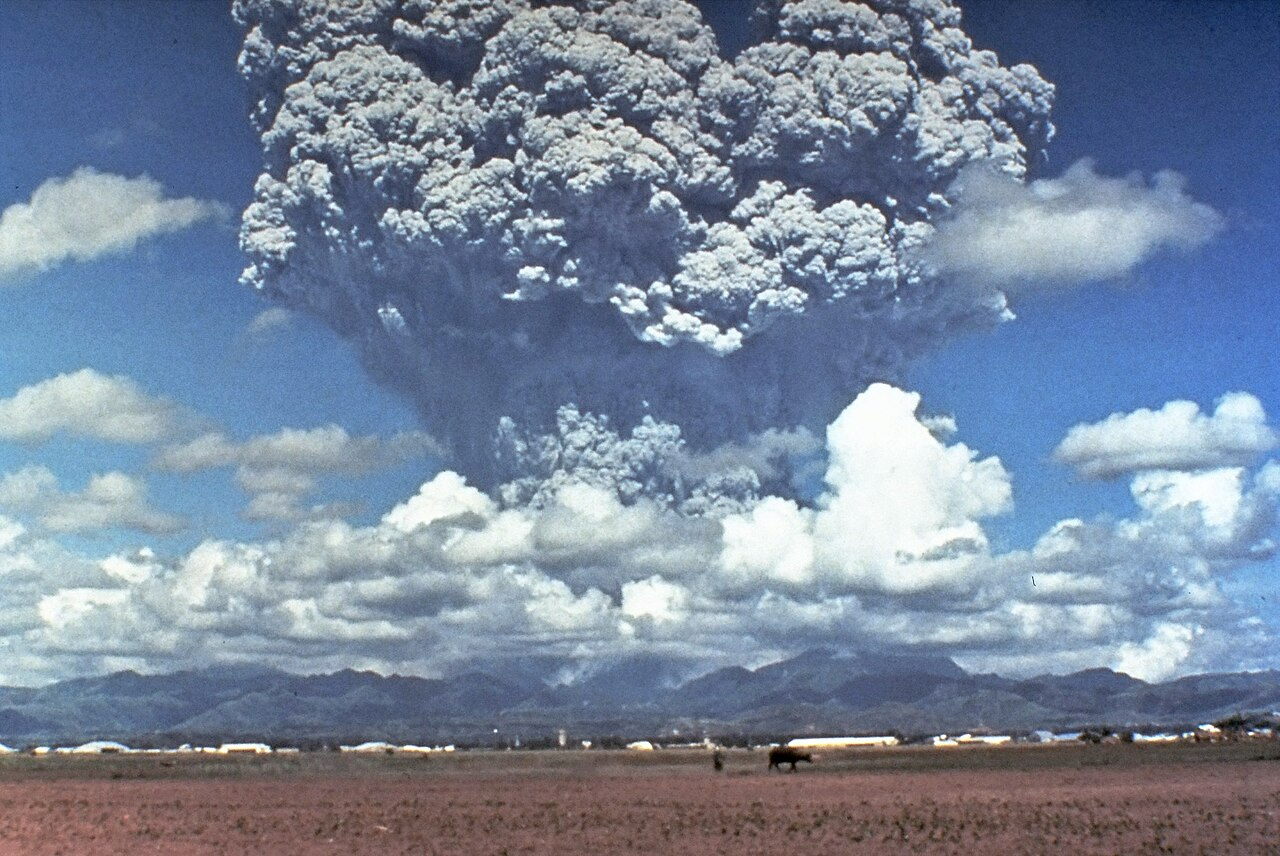
\includegraphics[height=4.5cm]{images/book1/g7-pinatubo.jpg}

{\small Eksplosif: tiang \omterm{def:g4:volcanoes-earthquakes-first-look:eruption}{letusan} Gunung Pinatubo, Filipina,
12~Juni 1991. Foto: Dave Harlow, USGS.}
\end{minipage}\par\medskip


{\small Kedua foto itu berada dalam domain publik (melalui Wikimedia
Commons).}
% ledger: commons:lava-fountain, commons:pinatubo
\label{fig:g7:volcanoes:two-photos}
\end{omfigure}

Apa yang membuat perbedaan itu? Dua hal: seberapa encer \omterm{def:g7:volcanoes:magma}{magmanya}, dan
seberapa banyak gas yang dikandungnya.

\textbf{Encer atau kental.} Sebagian \omterm{def:g7:volcanoes:magma}{magma} encer, hampir seperti madu
hangat: begitulah \omterm{def:g7:volcanoes:magma}{magma} yang mendingin menjadi basal gelap, seperti di
Hawaii. \omterm{def:g7:volcanoes:magma}{Magma} lain kental dan lengket, seperti madu dingin atau pasta gigi.
Di dalam \omterm{def:g7:volcanoes:magma}{magma} yang encer, gelembung-gelembung gas naik dengan mudah dan
lepas di permukaan, sedikit demi sedikit. Di dalam \omterm{def:g7:volcanoes:magma}{magma} yang kental,
gelembung-gelembung itu terperangkap.

\textbf{Sedikit atau banyak gas.} Sebotol air soda menyimpan banyak gas
yang terlarut di dalam airnya, yang tertahan di sana oleh tekanan di dalam
botol yang tertutup; kamu tidak dapat melihatnya. Bukalah botol itu, maka
tekanannya turun: gelembung-gelembung muncul di mana-mana, dan jika botol
itu sudah dikocok, buihnya menyembur keluar. \omterm{def:g7:volcanoes:magma}{Magma} yang jauh di bawah tanah
juga menyimpan gas yang terlarut di bawah tekanan tinggi. Ketika \omterm{def:g7:volcanoes:magma}{magma} itu
naik, tekanannya turun dan gas itu keluar dari larutan sebagai gelembung.
% ledger: usgs:volcanic-gases

Gabungkan keduanya. \omterm{def:g7:volcanoes:magma}{Magma} encer yang sedikit gasnya melepaskan
gelembung-gelembungnya dan keluar sebagai \omterm{def:g4:volcanoes-earthquakes-first-look:eruption}{lava} yang mengalir: \omterm{def:g4:volcanoes-earthquakes-first-look:eruption}{letusannya}
efusif. \omterm{def:g7:volcanoes:magma}{Magma} kental yang penuh gas menahan gelembung-gelembungnya sampai
gelembung itu begitu membesar sehingga mengoyak \omterm{def:g7:volcanoes:magma}{magma} menjadi
cabikan-cabikan: \omterm{def:g4:volcanoes-earthquakes-first-look:eruption}{letusannya} eksplosif. Cabikan \omterm{def:g7:volcanoes:magma}{magma} yang berbuih itu
membeku di udara menjadi abu dan menjadi batu apung, \omterm{def:g3:stones-pebbles-sand:rock}{batuan} yang begitu
penuh gelembung sehingga dapat terapung.

\begin{example}[Pinatubo, 1991: soda yang hambar dan soda yang dikocok]\label{ex:g7:volcanoes:pinatubo}
% ledger: usgs:pinatubo-1991
Pada bulan Juni~1991, \omterm{def:g7:volcanoes:magma}{magma} yang pertama mencapai permukaan Gunung
Pinatubo, di Filipina. Dalam perjalanannya ke atas, \omterm{def:g7:volcanoes:magma}{magma} itu sudah
kehilangan sebagian besar gasnya, ``seperti sebotol minuman soda yang sudah
hambar'', menurut kata-kata para ilmuwan yang mengamatinya. \omterm{def:g7:volcanoes:magma}{Magma} itu
merembes keluar perlahan-lahan dan menumpuk menjadi gundukan di atas \omterm{def:g7:volcanoes:vent}{lubang
letusan}: tidak ada ledakan. Kemudian, pada tanggal 12~Juni, \omterm{def:g7:volcanoes:magma}{magma} yang
masih penuh gas mencapai permukaan dan meledak --- itulah tiang \omterm{def:g4:volcanoes-earthquakes-first-look:eruption}{letusan}
pada foto di atas. Pada tanggal 15~Juni, datang \omterm{def:g7:volcanoes:magma}{magma} yang lebih kaya gas
lagi, dan \omterm{def:g4:volcanoes-earthquakes-first-look:volcano}{gunung api} itu mengalami salah satu \omterm{def:g4:volcanoes-earthquakes-first-look:eruption}{letusan} terbesar abad kedua
puluh: \omterm{def:g1:landscapes-around-us:landform}{gunung} itu memuntahkan lebih dari lima kilometer kubik \omterm{def:g3:stones-pebbles-sand:rock}{batuan} dan
abu, \omterm{def:g4:clouds-rain-snow:cloud}{awan} abunya naik setinggi \qty{35}{km}, dan puncak \omterm{def:g1:landscapes-around-us:landform}{gunung} itu runtuh
menjadi cekungan yang lebarnya \qty{2.5}{km}. \omterm{def:g4:volcanoes-earthquakes-first-look:volcano}{Gunung api} yang sama, pada
minggu yang sama: gaslah yang membuat perbedaan.
\end{example}

Bentuk sebuah \omterm{def:g4:volcanoes-earthquakes-first-look:volcano}{gunung api} menyimpan ingatan tentang \omterm{def:g4:volcanoes-earthquakes-first-look:eruption}{letusan-letusannya}.
\omterm{def:g4:volcanoes-earthquakes-first-look:eruption}{Lava} yang encer mengalir jauh sebelum mengeras, sehingga lapis demi lapis
\omterm{def:g4:volcanoes-earthquakes-first-look:eruption}{lava} itu membangun \omterm{def:g1:landscapes-around-us:landform}{gunung} yang lebar dengan lereng yang landai, berbentuk
seperti perisai prajurit yang tergeletak di tanah: \emph{\omterm{def:g4:volcanoes-earthquakes-first-look:volcano}{gunung api}
perisai}. Mauna Loa, di Hawaii, adalah salah satunya. \omterm{def:g4:volcanoes-earthquakes-first-look:eruption}{Lava} yang kental dan
abu menumpuk di dekat \omterm{def:g7:volcanoes:vent}{lubang letusan}, menjadi kerucut yang curam yang
tersusun atas lapisan-lapisan \omterm{def:g4:volcanoes-earthquakes-first-look:eruption}{lava} dan abu: \emph{\omterm{def:g4:volcanoes-earthquakes-first-look:volcano}{gunung api} strato}
(\emph{strata} berarti lapisan-lapisan). Gunung St.~Helens dan Pinatubo
adalah dua di antaranya.

\begin{omfigure}
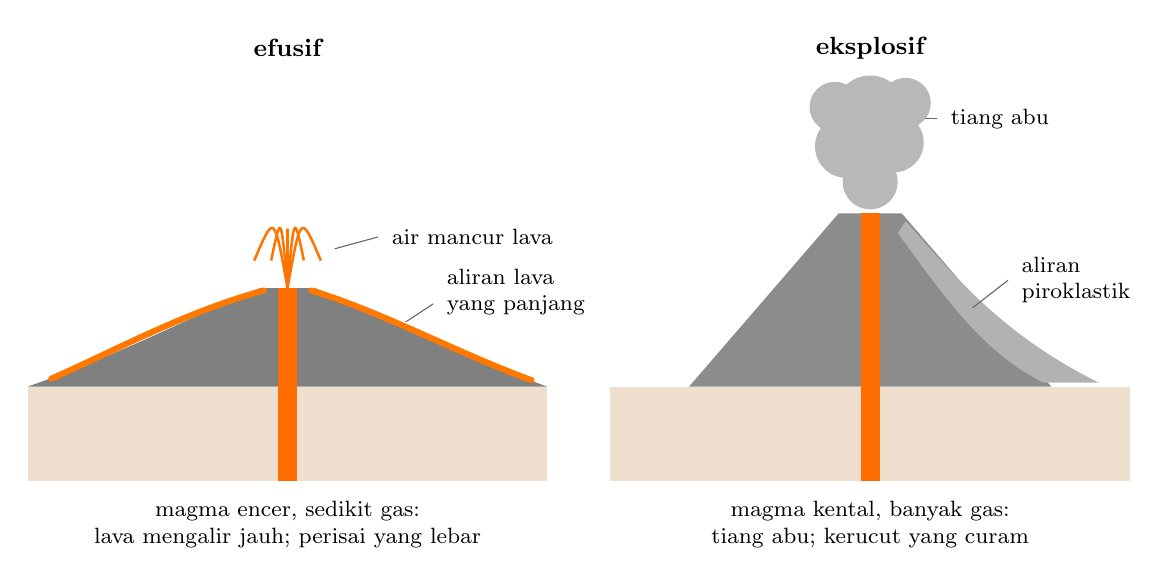
\begin{tikzpicture}[font=\small, x=1cm, y=1cm]
  % --- left: effusive, a shield
  \begin{scope}
    \fill[brown!25] (-3.3,-1.2) rectangle (3.3,0);
    \fill[black!50] (-3.3,0) .. controls (-2.0,0.45) and (-1.0,1.0) .. (-0.35,1.25)
      -- (0.35,1.25) .. controls (1.0,1.0) and (2.0,0.45) .. (3.3,0) -- cycle;
    \fill[orange!85!red] (-0.12,-1.2) rectangle (0.12,1.25);
    % fountain
    \foreach \a in {-25,-12,0,12,25}
      \draw[orange!90!red, line width=0.9pt] (0,1.25) .. controls ({0.4*sin(\a)},2.2) .. ({1.0*sin(\a)},1.6);
    % lava flows far down the gentle slopes
    \draw[orange!95!red, line width=2.2pt, line cap=round] (0.3,1.22) .. controls (1.2,0.95) and (2.1,0.45) .. (3.1,0.08);
    \draw[orange!95!red, line width=2.2pt, line cap=round] (-0.3,1.22) .. controls (-1.3,0.95) and (-2.2,0.45) .. (-3.0,0.1);
    \node[font=\small\bfseries] at (0,4.3) {efusif};
    \node[align=center, font=\footnotesize] at (0,-1.75) {magma encer, sedikit gas:\\lava mengalir jauh; perisai yang lebar};
    \node[anchor=west, font=\footnotesize] at (1.2,1.9) {air mancur lava};
    \draw[black!60] (1.15,1.9) -- (0.6,1.75);
    \node[anchor=west, font=\footnotesize, align=left] at (1.9,1.2) {aliran lava\\yang panjang};
    \draw[black!60] (1.85,1.05) -- (1.5,0.82);
  \end{scope}
  % --- right: explosive, a steep cone
  \begin{scope}[xshift=7.4cm]
    \fill[brown!25] (-3.3,-1.2) rectangle (3.3,0);
    \fill[black!45] (-2.3,0) -- (-0.4,2.2) -- (0.4,2.2) -- (2.3,0) -- cycle;
    \fill[orange!85!red] (-0.12,-1.2) rectangle (0.12,2.2);
    \foreach \x/\y/\r in {0/2.6/0.35, -0.3/3.05/0.4, 0.3/3.1/0.38, 0/3.5/0.45, -0.45/3.55/0.32, 0.45/3.6/0.32}
      \fill[black!28] (\x,\y) circle (\r);
    % pyroclastic flow down the flank
    \fill[black!30] (0.45,2.1) .. controls (1.0,1.5) and (1.6,0.7) .. (2.9,0.05)
      -- (2.2,0.05) .. controls (1.4,0.45) and (0.9,1.2) .. (0.35,1.95) -- cycle;
    \node[font=\small\bfseries] at (0,4.3) {eksplosif};
    \node[align=center, font=\footnotesize] at (0,-1.75) {magma kental, banyak gas:\\tiang abu; kerucut yang curam};
    \node[anchor=west, font=\footnotesize] at (0.9,3.4) {tiang abu};
    \draw[black!60] (0.85,3.4) -- (0.7,3.4);
    \node[anchor=west, font=\footnotesize, align=left] at (1.8,1.35) {aliran\\piroklastik};
    \draw[black!60] (1.75,1.35) -- (1.3,1.0);
  \end{scope}
\end{tikzpicture}

{\small Dua jenis \omterm{def:g4:volcanoes-earthquakes-first-look:eruption}{letusan} dan \omterm{def:g4:volcanoes-earthquakes-first-look:volcano}{gunung api} yang dibangunnya (gambar, tidak
berskala).}
\label{fig:g7:volcanoes:two-kinds}
\end{omfigure}

\begin{method}[Efusif atau eksplosif? Empat petunjuk]\label{met:g7:volcanoes:clues}
Untuk mengetahui dari sebuah uraian atau foto jenis \omterm{def:g4:volcanoes-earthquakes-first-look:eruption}{letusan} sebuah \omterm{def:g4:volcanoes-earthquakes-first-look:volcano}{gunung
api}, carilah petunjuk-petunjuk berikut.
\begin{enumerate}
  \item \emph{Apa yang keluar?} \omterm{def:g4:volcanoes-earthquakes-first-look:eruption}{Lava} yang mengalir atau menyembur sebagai
        air mancur: efusif. Tiang abu, bongkah \omterm{def:g3:stones-pebbles-sand:rock}{batuan} yang dilemparkan:
        eksplosif.
  \item \emph{Bentuk \omterm{def:g4:volcanoes-earthquakes-first-look:volcano}{gunung apinya}.} \omterm{def:g1:landscapes-around-us:landform}{Gunung} yang lebar dengan lereng yang
        landai: sebagian besar \omterm{def:g4:volcanoes-earthquakes-first-look:eruption}{letusannya} efusif. Kerucut yang curam: sering
        eksplosif.
  \item \emph{\omterm{def:g7:volcanoes:magma}{Magmanya}.} Encer, sedikit gas: efusif. Kental, banyak gas:
        eksplosif.
  \item \emph{\omterm{def:g3:stones-pebbles-sand:rock}{Batuan} yang ditinggalkan.} Aliran \omterm{def:g4:volcanoes-earthquakes-first-look:eruption}{lava} yang gelap dan padat:
        efusif. Lapisan-lapisan abu dan batu apung: eksplosif.
\end{enumerate}
\end{method}

\begin{example}[Memakai petunjuk-petunjuk itu]\label{ex:g7:volcanoes:clues}
Seorang pelancong menggambarkan sebuah \omterm{def:g4:volcanoes-earthquakes-first-look:volcano}{gunung api}: ``\omterm{def:g1:landscapes-around-us:landform}{gunung} yang sangat
besar dan membulat landai, aliran \omterm{def:g4:volcanoes-earthquakes-first-look:eruption}{lava} hitam di mana-mana di lerengnya,
sebagian baru berumur beberapa tahun''. Petunjuk~2 (lereng yang landai) dan
petunjuk~4 (aliran \omterm{def:g4:volcanoes-earthquakes-first-look:eruption}{lava} yang gelap) keduanya menunjuk ke \omterm{def:g7:volcanoes:eruption-types}{erupsi efusif}:
itulah \omterm{def:g4:volcanoes-earthquakes-first-look:volcano}{gunung api} perisai, seperti Mauna Loa.
\end{example}

\begin{inthelab}[Gunung api dalam botol (di kelas, bersama guru)]
Guru mengambil dua botol air soda yang tertutup. Botol yang satu dibiarkan
berdiri; botol yang lain dikocok perlahan. Keduanya dibuka di luar ruangan,
di atas sebuah baskom, dengan mulut botol diarahkan menjauhi semua orang.
Botol yang diam mendesis dan melepaskan beberapa gelembung; botol yang
dikocok menyemburkan buih. Botol mana yang seperti \omterm{def:g7:volcanoes:magma}{magma} Hawaii, dan botol
mana yang seperti \omterm{def:g7:volcanoes:magma}{magma} Pinatubo? Lalu masukkan sepotong batu apung dan
sebutir \omterm{def:g3:stones-pebbles-sand:pebble}{kerikil} ke dalam semangkuk air: batu apungnya terapung. Amatilah
batu apung itu dengan kaca pembesar: batu itu penuh lubang, yaitu
gelembung-gelembung gas yang membeku di dalam \omterm{def:g3:stones-pebbles-sand:rock}{batuan} ketika \omterm{def:g7:volcanoes:magma}{magmanya}
meledak.
\end{inthelab}

\section{Apa yang keluar dari gunung api}

Sebuah \omterm{def:g4:volcanoes-earthquakes-first-look:eruption}{letusan} memuntahkan jauh lebih banyak daripada \omterm{def:g4:volcanoes-earthquakes-first-look:eruption}{lava}: gas, abu,
bongkah \omterm{def:g3:stones-pebbles-sand:rock}{batuan}, dan, dalam keadaan yang paling buruk, longsoran abu panas.

Gas yang paling banyak, jauh melebihi yang lain, adalah uap air.
\omterm{def:g4:volcanoes-earthquakes-first-look:eruption}{Letusan-letusan} besar melepaskan gas dalam jumlah sangat besar dalam waktu
singkat: dalam satu hari saja pada tahun 1991, Pinatubo diperkirakan telah
mengirimkan lebih dari 250~juta ton gas ke atmosfer atas.
% ledger: usgs:volcanic-gases

\begin{definition}[Aliran piroklastik]\label{def:g7:volcanoes:pyroclastic-flow}
Yang disebut \emph{aliran piroklastik}\index{aliran piroklastik} adalah
longsoran cepat dari gas panas, abu, dan pecahan \omterm{def:g3:stones-pebbles-sand:rock}{batuan}, mulai dari butir
debu sampai bongkah besar, yang meluncur deras menuruni lereng \omterm{def:g4:volcanoes-earthquakes-first-look:volcano}{gunung api}
ketika \omterm{def:g7:volcanoes:eruption-types}{erupsi eksplosif}. (\emph{Piro} berarti api dan \emph{klastik} berarti
terdiri atas pecahan-pecahan.)
\end{definition}

\omterm{def:g7:volcanoes:pyroclastic-flow}{Aliran piroklastik} biasanya bergerak lebih cepat daripada \qty{80}{km/h},
dan \omterm{def:g3:stones-pebbles-sand:rock}{batuan} serta gas di dalamnya umumnya bersuhu antara 200 dan
\qty{700}{\degreeCelsius}. Aliran ini umumnya mengikuti \omterm{def:g1:landscapes-around-us:landform}{lembah}, seperti air,
dan merobohkan, membakar, atau mengubur hampir segala sesuatu di jalannya.
Pada tanggal 18~Mei 1980, \omterm{def:g7:volcanoes:pyroclastic-flow}{aliran piroklastik} Gunung St.~Helens melaju
dengan kecepatan 80 sampai \qty{130}{km/h}, pada suhu paling sedikit
\qty{700}{\degreeCelsius}, dan mencapai jarak \qty{8}{km} dari \omterm{def:g7:volcanoes:vent}{kawah}.
% ledger: usgs:pyroclastic-flows, usgs:msh-flows, usgs:msh-reach

Tabel berikut merangkum hasil-hasil \omterm{def:g4:volcanoes-earthquakes-first-look:eruption}{letusan} \omterm{def:g4:volcanoes-earthquakes-first-look:volcano}{gunung api}.

\begin{center}
\small
\begin{tabular}{|p{0.2\linewidth}|p{0.4\linewidth}|p{0.3\linewidth}|}
\hline
\textbf{hasil} & \textbf{apakah itu} & \textbf{bahayanya} \\
\hline
aliran \omterm{def:g4:volcanoes-earthquakes-first-look:eruption}{lava} & \omterm{def:g3:stones-pebbles-sand:rock}{batuan} cair yang mengalir di tanah, lalu mengeras & membakar dan mengubur apa yang ditemuinya, tetapi biasanya cukup lambat sehingga orang sempat menyingkir \\
\hline
abu & kepingan-kepingan kecil \omterm{def:g3:stones-pebbles-sand:rock}{batuan} dan kaca, yang dihembuskan ke udara & jatuh di tempat yang jauh; atap runtuh karena beratnya; merusak pesawat terbang \\
\hline
bom vulkanik & gumpalan \omterm{def:g4:volcanoes-earthquakes-first-look:eruption}{lava} yang dilemparkan, yang mengeras selagi melayang & menghancurkan apa yang ditimpanya, di dekat \omterm{def:g7:volcanoes:vent}{lubang letusan} \\
\hline
gas & terutama uap air, lalu karbon dioksida dan sulfur dioksida & sebagian beracun; karbon dioksida berkumpul di cekungan-cekungan \\
\hline
\omterm{def:g7:volcanoes:pyroclastic-flow}{aliran piroklastik} & longsoran abu panas, \omterm{def:g3:stones-pebbles-sand:rock}{batuan}, dan gas & yang paling mematikan: terlalu cepat dan terlalu panas untuk dihindari \\
\hline
aliran lumpur & abu dan \omterm{def:g3:stones-pebbles-sand:rock}{batuan} yang bercampur dengan air \omterm{def:g4:clouds-rain-snow:precipitation}{hujan} atau \omterm{def:g4:clouds-rain-snow:precipitation}{salju} yang mencair & meluncur deras menuruni \omterm{def:g1:landscapes-around-us:landform}{lembah}, kadang-kadang jauh dari \omterm{def:g4:volcanoes-earthquakes-first-look:volcano}{gunung api} \\
\hline
\end{tabular}
\end{center}
% ledger: usgs:lava-flows, usgs:volcanic-gases, usgs:pyroclastic-flows, usgs:pinatubo-1991, usgs:msh-flows

\begin{method}[Berapa lama waktunya?]\label{met:g7:volcanoes:time}
Untuk mengetahui berapa lama sesuatu yang bergerak dengan kecepatan yang
diketahui menempuh suatu jarak, bagilah jarak itu dengan kecepatannya:
\[
\text{waktu} = \frac{\text{jarak}}{\text{kecepatan}}.
\]
Dengan jarak dalam kilometer dan kecepatan dalam kilometer per jam, waktu
yang didapat dalam jam; kalikan dengan 60 untuk mendapatkan menit.
\end{method}

\begin{example}[Berlomba dengan aliran piroklastik]\label{ex:g7:volcanoes:race}
Sebuah \omterm{def:g7:volcanoes:pyroclastic-flow}{aliran piroklastik} yang bergerak dengan kecepatan \qty{120}{km/h}
menuju sebuah desa yang terletak \qty{6}{km} di hilir \omterm{def:g1:landscapes-around-us:landform}{lembah}. Aliran itu
memerlukan $6 \div 120 = 0.05$~jam, yaitu $0.05 \times 60 = 3$~menit. Tiga
menit: tidak ada orang yang dapat berlari, atau bahkan mengemudi, keluar
dari \omterm{def:g1:landscapes-around-us:landform}{lembah} itu tepat waktu. Orang hanya selamat jika mereka sudah pergi
\emph{sebelum} \omterm{def:g4:volcanoes-earthquakes-first-look:eruption}{letusan}.
\end{example}

\begin{remark}[Aliran lumpur: bahaya yang datang kemudian]\label{rem:g7:volcanoes:mudflows}
% ledger: usgs:msh-flows, usgs:pinatubo-lahars
Sebuah \omterm{def:g4:volcanoes-earthquakes-first-look:eruption}{letusan} meninggalkan lereng yang tertutup abu yang lepas. Ketika
\omterm{def:g4:clouds-rain-snow:precipitation}{hujan} turun di atasnya, atau ketika panasnya mencairkan \omterm{def:g4:clouds-rain-snow:precipitation}{salju} dan es di
puncak, abu itu berubah menjadi aliran lumpur yang meluncur deras menuruni
\omterm{def:g1:landscapes-around-us:landform}{lembah}. Pada tanggal 18~Mei 1980, aliran lumpur Gunung St.~Helens merusak
27~jembatan dan hampir 200~rumah. Di sekitar Pinatubo, \omterm{def:g4:clouds-rain-snow:precipitation}{hujan} lebat pada
tahun-tahun berikutnya mengubah abu itu menjadi aliran lumpur raksasa yang
mengubur seluruh desa: kerusakannya lebih besar daripada kerusakan akibat
\omterm{def:g4:volcanoes-earthquakes-first-look:eruption}{letusan} itu sendiri.
\end{remark}


\section{Di mana letak gunung-gunung api?}

Smithsonian Institution, di Washington, menyimpan daftar semua \omterm{def:g4:volcanoes-earthquakes-first-look:volcano}{gunung api}
yang diketahui telah meletus dalam 12\,000 tahun terakhir: 1\,214 \omterm{def:g4:volcanoes-earthquakes-first-look:volcano}{gunung
api}, di darat maupun di bawah \omterm{def:g2:water-on-earth:ocean}{laut}. Untuk setiap \omterm{def:g4:volcanoes-earthquakes-first-look:volcano}{gunung api}, daftar itu
menyebutkan letaknya terhadap \omterm{def:g7:plate-tectonics:plate}{lempeng-lempeng}. \omterm{def:g2:drawing-to-map:map}{Peta} di bawah ini
mewarnainya dengan cara itu.
% ledger: data:gvp (counts computed in figdata/grade-7/volcano_settings.py)

\begin{omfigure}
\begin{tikzpicture}
\begin{axis}[ommap, width=\linewidth, xtick={-180,-90,...,180}, ytick={-60,0,60},
  legend style={at={(0.02,0.04)}, anchor=south west, font=\scriptsize,
  fill=white, fill opacity=0.85, text opacity=1, draw=black!40}, legend cell align=left]
\addplot[fill=omLithAlluv, draw=black!45, line width=0.2pt, forget plot] table {figdata/out/shared-geo-land.dat};
\addplot[omRidge!60, line width=0.5pt, forget plot] table {figdata/out/shared-geo-school-ridge.dat};
\addplot[omTrench!60, line width=0.5pt, forget plot] table {figdata/out/shared-geo-school-subduction.dat};
\addplot[only marks, mark=triangle*, mark size=1.3pt, omTrench, forget plot] table {figdata/out/grade-7-volcano_settings-map-sub.dat};
\addplot[only marks, mark=triangle*, mark size=1.3pt, omRidge, forget plot] table {figdata/out/grade-7-volcano_settings-map-rift.dat};
\addplot[only marks, mark=*, mark size=1.4pt, orange!90!black, forget plot] table {figdata/out/grade-7-volcano_settings-map-intra.dat};
\addlegendimage{only marks, mark=triangle*, mark size=1.6pt, omTrench}
\addlegendentry{tempat satu lempeng menunjam ke bawah lempeng lain}
\addlegendimage{only marks, mark=triangle*, mark size=1.6pt, omRidge}
\addlegendentry{tempat lempeng-lempeng saling menjauh}
\addlegendimage{only marks, mark=*, mark size=1.6pt, orange!90!black}
\addlegendentry{di dalam lempeng}
\end{axis}
\end{tikzpicture}

{\small \omterm{def:g4:volcanoes-earthquakes-first-look:volcano}{Gunung-gunung api} yang aktif dalam 12\,000 tahun terakhir, diwarnai
menurut letaknya. Garis-garis tipis: \omterm{def:g7:plate-tectonics:plate-boundary}{batas lempeng} tempat \omterm{def:g7:plate-tectonics:plate}{lempeng-lempeng}
saling menjauh (merah) dan tempat satu \omterm{def:g7:plate-tectonics:plate}{lempeng} menunjam ke bawah \omterm{def:g7:plate-tectonics:plate}{lempeng}
lain (biru). Data: Smithsonian Global Volcanism Program; \omterm{def:g7:plate-tectonics:plate-boundary}{batas lempeng}
menurut P.~Bird (2003); garis pantai dari Natural Earth.}
% ledger: data:gvp, data:pb2002, data:ne-land
\label{fig:g7:volcanoes:map}
\end{omfigure}

\begin{omfigure}
\begin{tikzpicture}
  \begin{axis}[xbar, width=0.64\linewidth, height=3.6cm, bar width=8pt,
      xmin=0, xmax=1000, ymin=-0.6, ymax=3.6, y dir=reverse,
      ytick={0,...,3}, yticklabels={tempat satu lempeng menunjam, tempat lempeng saling menjauh, di dalam lempeng, tidak diketahui},
      xlabel={jumlah gunung api},
      axis x line=bottom, axis y line=left, axis line style={-},
      tick label style={font=\scriptsize}, label style={font=\small},
      nodes near coords, nodes near coords style={font=\scriptsize, anchor=west},
      point meta=explicit symbolic, enlarge y limits=false, clip=false]
    \addplot[fill=black!30, draw=black!60] table[x=n, y=idx, meta=n] {figdata/out/grade-7-volcano_settings.dat};
  \end{axis}
\end{tikzpicture}

{\small Berapa banyak dari 1\,214 \omterm{def:g4:volcanoes-earthquakes-first-look:volcano}{gunung api} itu yang terletak di setiap tatanan.}
% ledger: data:gvp (figdata/grade-7/volcano_settings.py, main table)
\label{fig:g7:volcanoes:counts}
\end{omfigure}

\begin{proposition}[Sebagian besar gunung api terletak di batas lempeng]\label{prop:g7:volcanoes:where}
% ledger: data:gvp (counts computed in figdata/grade-7/volcano_settings.py)
Dari 1\,214 \omterm{def:g4:volcanoes-earthquakes-first-look:volcano}{gunung api} yang aktif dalam 12\,000 tahun terakhir, 838
(69~\%) terletak di tempat satu \omterm{def:g7:plate-tectonics:plate}{lempeng} menunjam ke bawah \omterm{def:g7:plate-tectonics:plate}{lempeng} lain dan
221 (18~\%) di tempat \omterm{def:g7:plate-tectonics:plate}{lempeng-lempeng} saling menjauh; 149 (12~\%) terletak
di dalam \omterm{def:g7:plate-tectonics:plate}{lempeng}, jauh dari tepinya. Untuk 6 sisanya (0.5~\%), tatanannya
tidak diketahui.
\end{proposition}

\textbf{Tempat \omterm{def:g7:plate-tectonics:plate}{lempeng-lempeng} saling menjauh.} Di sepanjang punggung
\omterm{def:g2:water-on-earth:ocean}{samudra}, dan di rekahan seperti rekahan yang sedang membelah Afrika Timur,
\omterm{def:g7:plate-tectonics:plate}{lempeng-lempeng} saling menarik menjauh. \omterm{def:g7:volcanoes:magma}{Magma} naik dari \omterm{def:g6:inside-the-earth:layers}{mantel} ke dalam
retakan-retakan yang makin lebar dan mengisinya: \omterm{def:g6:inside-the-earth:layers}{kerak} baru terbentuk.
Sebagian besar punggung \omterm{def:g2:water-on-earth:ocean}{samudra} terletak di bawah \omterm{def:g2:water-on-earth:ocean}{laut}, tetapi Islandia
berdiri tepat di atas Punggung Tengah Atlantik: di sana \omterm{def:g4:volcanoes-earthquakes-first-look:volcano}{gunung-gunung api}
ini dapat dilihat di darat. \omterm{def:g7:volcanoes:magma}{Magmanya} sebagian besar basal yang encer, dan
\omterm{def:g4:volcanoes-earthquakes-first-look:eruption}{letusannya} sebagian besar efusif.
% ledger: usgs:arc-magma, usgs:iceland, usgs:east-africa

\textbf{Tempat satu \omterm{def:g7:plate-tectonics:plate}{lempeng} menunjam ke bawah \omterm{def:g7:plate-tectonics:plate}{lempeng} lain.} Lebih dari
dua dari setiap tiga \omterm{def:g4:volcanoes-earthquakes-first-look:volcano}{gunung api} terletak di sini, di sepanjang garis-garis
yang mengikuti tepi \omterm{def:g2:water-on-earth:ocean}{Samudra} Pasifik --- ``Cincin Api'' --- dan di beberapa
tempat lain. Jauh di bawah, di sepanjang \omterm{def:g7:plate-tectonics:plate}{lempeng} yang menunjam, sebagian
\omterm{def:g3:stones-pebbles-sand:rock}{batuan} meleleh sebagian; para ilmuwan masih memperdebatkan \omterm{def:g3:stones-pebbles-sand:rock}{batuan} mana
persisnya yang meleleh, \omterm{def:g7:plate-tectonics:plate}{lempeng} yang menunjam atau \omterm{def:g7:plate-tectonics:plate}{lempeng} di atasnya, atau
keduanya. \omterm{def:g7:volcanoes:magma}{Magma} yang naik di sana sering kental dan penuh gas: inilah
\omterm{def:g4:volcanoes-earthquakes-first-look:volcano}{gunung-gunung api} yang eksplosif, seperti Gunung St.~Helens dan Pinatubo.
Data menunjukkannya: dari 660 kerucut curam (\omterm{def:g4:volcanoes-earthquakes-first-look:volcano}{gunung api} strato) dalam
daftar itu, 564 --- yaitu 85~\% --- terletak di tempat satu \omterm{def:g7:plate-tectonics:plate}{lempeng}
menunjam ke bawah \omterm{def:g7:plate-tectonics:plate}{lempeng} lain.
% ledger: usgs:arc-magma, data:gvp (figdata/grade-7/volcano_settings.py, part strato)

\textbf{Di dalam \omterm{def:g7:plate-tectonics:plate}{lempeng}.} Beberapa \omterm{def:g4:volcanoes-earthquakes-first-look:volcano}{gunung api} terletak jauh dari batas mana
pun. Yang paling terkenal adalah \omterm{def:g4:volcanoes-earthquakes-first-look:volcano}{gunung-gunung api} di Hawaii, di
tengah-tengah \omterm{def:g2:water-on-earth:ocean}{Samudra} Pasifik, lebih dari \qty{3200}{km} dari tepi \omterm{def:g7:plate-tectonics:plate}{lempeng}
yang terdekat.
% ledger: usgs:hawaii-hotspot

\begin{definition}[Titik panas]\label{def:g7:volcanoes:hotspot}
Yang disebut \emph{titik panas}\index{titik panas} adalah suatu tempat, jauh
di dalam \omterm{def:g6:inside-the-earth:layers}{mantel}, yang tetap panas selama jutaan tahun dan terus memasok
\omterm{def:g7:volcanoes:magma}{magma} ke \omterm{def:g4:volcanoes-earthquakes-first-look:volcano}{gunung-gunung api} di permukaan, bahkan jauh dari tepi \omterm{def:g7:plate-tectonics:plate}{lempeng}.
\end{definition}

\omterm{def:g7:volcanoes:hotspot}{Titik panas} itu tetap di tempatnya, sedangkan \omterm{def:g7:plate-tectonics:plate}{lempeng} di atasnya bergerak.
Sebuah \omterm{def:g4:volcanoes-earthquakes-first-look:volcano}{gunung api} tumbuh di atas \omterm{def:g7:volcanoes:hotspot}{titik panas}; lalu \omterm{def:g7:plate-tectonics:plate}{lempeng} yang bergerak
membawanya pergi, dan \omterm{def:g4:volcanoes-earthquakes-first-look:volcano}{gunung api} itu mati, sementara \omterm{def:g4:volcanoes-earthquakes-first-look:volcano}{gunung api} baru tumbuh
di atas \omterm{def:g7:volcanoes:hotspot}{titik panas} di belakangnya. Lama-kelamaan, \omterm{def:g7:plate-tectonics:plate}{lempeng} itu membawa
sederet \omterm{def:g4:volcanoes-earthquakes-first-look:volcano}{gunung api}, yang paling tua paling jauh dari \omterm{def:g7:volcanoes:hotspot}{titik panas}. Itulah
tepatnya yang kita lihat di Hawaii: \omterm{def:g3:stones-pebbles-sand:rock}{batuan} tertua di Pulau Kauai, di ujung
barat laut pulau-pulau yang berpenghuni, berumur kira-kira 5.5~juta tahun,
dan sudah sangat terkikis oleh \omterm{def:g4:clouds-rain-snow:precipitation}{hujan} dan ombak; di Pulau Besar (pulau
Hawaii yang terbesar), di ujung tenggara, \omterm{def:g3:stones-pebbles-sand:rock}{batuan} tertua di permukaan berumur kurang dari
0.7~juta tahun, dan \omterm{def:g4:volcanoes-earthquakes-first-look:eruption}{lava} baru masih keluar.
% ledger: usgs:hawaii-hotspot

\begin{history}[Seorang ahli geofisika dan sederet pulau]
% ledger: usgs:hawaii-hotspot
Mengapa serangkaian pulau \omterm{def:g4:volcanoes-earthquakes-first-look:volcano}{gunung api} muncul di tengah-tengah \omterm{def:g7:plate-tectonics:plate}{lempeng}
terbesar di Bumi? Pada tahun 1963, ahli geofisika Kanada J.~Tuzo Wilson
mengajukan sebuah jawaban. Menurutnya, pulau-pulau Hawaii berderet karena
\omterm{def:g7:plate-tectonics:plate}{lempeng} Pasifik bergerak di atas sumber panas yang dalam dan tetap di
dalam \omterm{def:g6:inside-the-earth:layers}{mantel}, yang melelehkan sebagian \omterm{def:g7:plate-tectonics:plate}{lempeng} di atasnya. Jika ia benar,
pulau-pulau itu seharusnya makin tua dan makin terkikis makin jauh letaknya
dari \omterm{def:g4:volcanoes-earthquakes-first-look:volcano}{gunung-gunung api} yang aktif di Pulau Besar. Umur \omterm{def:g3:stones-pebbles-sand:rock}{batuannya}
menunjukkan tepat hal itu. Satu gagasan saja menjelaskan baik deretnya maupun urutan umurnya.
(Wilson juga ilmuwan yang menemukan \omterm{def:g7:plate-tectonics:plate-boundary}{batas transform}, tempat \omterm{def:g7:plate-tectonics:plate}{lempeng-lempeng}
saling bergeser berpapasan.)
\end{history}

\begin{omfigure}
\begin{tikzpicture}[font=\small, x=1cm, y=1cm]
  % sea, plate and mantle
  \fill[omSea!45] (-6.2,0) rectangle (6.2,1.0);
  \fill[orange!12] (-6.2,-3.4) rectangle (6.2,-1.0);
  \fill[brown!35] (-6.2,-1.0) rectangle (6.2,0);
  \draw[omSea!80!black, line width=0.5pt] (-6.2,1.0) -- (6.2,1.0);
  \node[font=\footnotesize] at (-4.6,-0.5) {lempeng Pasifik};
  % the hotspot plume, fixed in the mantle, and the magma rising to the volcano
  \fill[orange!80!red] (4.0,-3.4) .. controls (3.6,-2.4) .. (3.75,-1.0) -- (4.25,-1.0) .. controls (4.4,-2.4) .. (4.0,-3.4) -- cycle;
  \node[anchor=west, align=left, font=\footnotesize] at (4.5,-2.5) {titik panas: tetap\\di tempatnya};
  % volcanoes rise from the sea floor; youngest over the hotspot
  \fill[black!55] (2.3,0) .. controls (3.2,1.2) .. (3.75,1.85) -- (4.25,1.85) .. controls (4.8,1.2) .. (5.7,0) -- cycle;
  \fill[orange!80!red] (3.93,-1.0) rectangle (4.07,1.85);
  \fill[black!45] (-0.4,0) .. controls (0.4,0.9) .. (0.9,1.3) -- (1.3,1.3) .. controls (1.8,0.9) .. (2.6,0) -- cycle;
  \fill[black!35] (-3.2,0) .. controls (-2.5,0.6) .. (-2.1,0.8) -- (-1.7,0.8) .. controls (-1.3,0.6) .. (-0.6,0) -- cycle;
  \fill[black!28] (-5.8,0) .. controls (-5.2,0.4) .. (-4.9,0.5) -- (-4.6,0.5) .. controls (-4.3,0.4) .. (-3.6,0) -- cycle;
  % labels
    \node[align=center, font=\footnotesize, anchor=south] at (4.3,1.95) {gunung api aktif\\(Pulau Besar: kurang\\dari 0.7 juta tahun)};
  \node[align=center, font=\footnotesize, anchor=south] at (0.7,1.4) {pulau tua yang terkikis\\(Kauai: kira-kira\\5.5 juta tahun)};
  \node[align=center, font=\footnotesize] at (-1.9,1.5) {gunung api yang lebih tua,\\di bawah ombak};
  \node[align=center, font=\footnotesize] at (-4.75,1.3) {lebih tua lagi,\\tenggelam};
  \node[font=\footnotesize] at (5.75,0.55) {laut};
  \node[font=\footnotesize] at (-4.3,-2.2) {mantel};
  % plate motion
  \draw[-{Stealth[length=3mm]}, line width=1.2pt] (2.2,-0.62) -- (-1.8,-0.62);
  \node[font=\footnotesize] at (0.2,-0.28) {lempeng bergerak ke barat laut};
    \node[font=\footnotesize\bfseries] at (-5.8,-3.1) {BL};
  \node[font=\footnotesize\bfseries] at (5.8,-3.1) {TG};
\end{tikzpicture}

{\small Sebuah \omterm{def:g7:plate-tectonics:plate}{lempeng} yang bergerak di atas \omterm{def:g7:volcanoes:hotspot}{titik panas} (gambar, tidak
berskala; pulau-pulau di antaranya tidak digambar). \omterm{def:g4:volcanoes-earthquakes-first-look:volcano}{Gunung api} di atas
\omterm{def:g7:volcanoes:hotspot}{titik panas} masih muda dan aktif; \omterm{def:g7:plate-tectonics:plate}{lempeng} membawa \omterm{def:g4:volcanoes-earthquakes-first-look:volcano}{gunung-gunung api} yang
lebih tua ke arah barat laut, tempat \omterm{def:g4:volcanoes-earthquakes-first-look:volcano}{gunung-gunung api} itu mati, terkikis,
dan akhirnya tenggelam di bawah ombak.}
% ledger: usgs:hawaii-hotspot
\label{fig:g7:volcanoes:hotspot}
\end{omfigure}

\begin{omfigure}
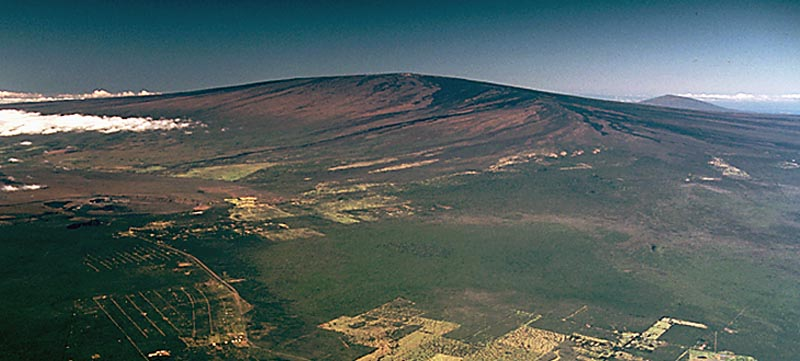
\includegraphics[width=0.8\linewidth]{images/book1/g7-mauna-loa.jpg}

{\small Mauna Loa, \omterm{def:g4:volcanoes-earthquakes-first-look:volcano}{gunung api} perisai di Pulau Besar Hawaii, dilihat dari
udara: \omterm{def:g1:landscapes-around-us:landform}{gunung} yang sangat besar dengan lereng yang landai, yang dibangun
oleh ribuan aliran \omterm{def:g4:volcanoes-earthquakes-first-look:eruption}{lava} yang encer. Foto: J.~D. Griggs, U.S. Geological
Survey, 1985 (domain publik, melalui Wikimedia Commons).}
% ledger: commons:mauna-loa
\label{fig:g7:volcanoes:mauna-loa}
\end{omfigure}

\section{Hidup berdampingan dengan gunung api}

Banyak orang tinggal di dekat \omterm{def:g4:volcanoes-earthquakes-first-look:volcano}{gunung api}: kira-kira 3~juta orang tinggal di
wilayah sekitar Pinatubo pada tahun 1991. Untunglah, \omterm{def:g4:volcanoes-earthquakes-first-look:eruption}{letusan} besar sering
memberikan tanda-tanda peringatan. \omterm{def:g7:volcanoes:magma}{Magma} yang naik mendorong \omterm{def:g3:stones-pebbles-sand:rock}{batuan} ke
samping: tanah retak dan berguncang oleh gempa-gempa bumi kecil, lerengnya
menggembung, gas keluar. Di Gunung St.~Helens, \omterm{def:g4:volcanoes-earthquakes-first-look:earthquake}{gempa bumi} kecil yang
pertama terjadi pada tanggal 16~Maret 1980; sampai tanggal 17~Mei, sudah
terjadi lebih dari 10\,000 gempa, dan lereng utaranya sudah menggembung ke
luar paling sedikit \qty{137}{m}. Para ilmuwan mengukur semua ini dan
kawasan itu ditutup; walaupun begitu, 57~orang tewas pada tanggal 18~Mei.
% ledger: usgs:msh-lead-up, usgs:msh-flows

Di Pinatubo, pada tahun 1991, para ilmuwan yang mengamati gempa-gempa bumi,
gas, dan penggembungan \omterm{def:g4:volcanoes-earthquakes-first-look:volcano}{gunung api} itu memberikan peringatan tepat waktu:
orang-orang yang tinggal di dekat \omterm{def:g4:volcanoes-earthquakes-first-look:volcano}{gunung api} itu mengungsi, dan paling
sedikit 5\,000 jiwa terselamatkan.
% ledger: usgs:pinatubo-1991 (central Luzon home to about 3 million people)

\begin{remark}[Jangan pernah mendekati gunung api yang sedang meletus]\label{rem:g7:volcanoes:safety}
Menyaksikan \omterm{def:g4:volcanoes-earthquakes-first-look:eruption}{letusan} hanya boleh dilakukan di tempat-tempat yang sudah
dibuka untuk umum oleh pihak berwenang. Gas, batu yang berjatuhan, \omterm{def:g6:inside-the-earth:layers}{kerak}
\omterm{def:g4:volcanoes-earthquakes-first-look:eruption}{lava} baru yang pecah di bawah kakimu, dan \omterm{def:g7:volcanoes:pyroclastic-flow}{aliran piroklastik} dapat
membunuh, sering tanpa peringatan. Pos-pos pengamatan \omterm{def:g4:volcanoes-earthquakes-first-look:volcano}{gunung api}
mengumumkan tempat-tempat yang aman untuk dikunjungi: selalu ikutilah
petunjuknya.
\end{remark}

\section{Latihan}

\begin{exercise}[$\star$]\label{exo:g7:volcanoes:1}
Pasangkan setiap kata dengan artinya: \omterm{def:g7:volcanoes:magma}{magma}; \omterm{def:g4:volcanoes-earthquakes-first-look:eruption}{lava}; \omterm{def:g7:volcanoes:magma-chamber}{dapur magma}; \omterm{def:g7:volcanoes:vent}{lubang
letusan}; \omterm{def:g7:volcanoes:vent}{kawah}. (a) Cekungan berbentuk mangkuk di puncak \omterm{def:g4:volcanoes-earthquakes-first-look:volcano}{gunung api}.
(b) \omterm{def:g3:stones-pebbles-sand:rock}{Batuan} cair di bawah tanah. (c) Bukaan tempat \omterm{def:g7:volcanoes:magma}{magma} keluar. (d) \omterm{def:g3:stones-pebbles-sand:rock}{Batuan}
cair yang sudah keluar ke permukaan. (e) Kantong \omterm{def:g7:volcanoes:magma}{magma} yang besar beberapa
kilometer di bawah \omterm{def:g4:volcanoes-earthquakes-first-look:volcano}{gunung api}.
\end{exercise}

\begin{exercise}[$\star$]\label{exo:g7:volcanoes:2}
Efusif atau eksplosif? (a) \omterm{def:g1:landscapes-around-us:water}{Sungai-sungai} \omterm{def:g4:volcanoes-earthquakes-first-look:eruption}{lava} berpijar mengalir menuruni
lereng yang landai. (b) Tiang abu naik setinggi \qty{35}{km} ke langit.
(c) Air mancur tetes-tetes berpijar menyembur dari sebuah retakan.
(d) Longsoran abu panas dan gas meluncur deras menuruni \omterm{def:g1:landscapes-around-us:landform}{lembah}.
\end{exercise}

\begin{exercise}[$\star$]\label{exo:g7:volcanoes:3}
Benar atau salah? Perbaikilah pernyataan yang salah. (a) \omterm{def:g7:volcanoes:magma}{Magma} dan \omterm{def:g4:volcanoes-earthquakes-first-look:eruption}{lava}
adalah dua nama untuk \omterm{def:g3:stones-pebbles-sand:rock}{batuan} cair yang sama, di bawah tanah dan di
permukaan. (b) Gas \omterm{def:g4:volcanoes-earthquakes-first-look:volcano}{gunung api} yang paling banyak adalah karbon dioksida.
(c) \omterm{def:g7:volcanoes:pyroclastic-flow}{Aliran piroklastik} adalah \omterm{def:g1:landscapes-around-us:water}{sungai} \omterm{def:g4:volcanoes-earthquakes-first-look:eruption}{lava} cair. (d) \omterm{def:g4:volcanoes-earthquakes-first-look:volcano}{Gunung-gunung api}
Hawaii terletak di \omterm{def:g7:plate-tectonics:plate-boundary}{batas lempeng}.
\end{exercise}

\begin{exercise}[$\star$]\label{exo:g7:volcanoes:4}
Gunakan tabel warna pijar. (a) \omterm{def:g4:volcanoes-earthquakes-first-look:eruption}{Lava} berpijar kuning: sebutkan suhunya.
(b) Aliran yang sedang mengeras berpijar merah tua: sebutkan suhunya.
(c) Sebuah foto menunjukkan \omterm{def:g4:volcanoes-earthquakes-first-look:eruption}{lava} oranye di bagian depan aliran dan \omterm{def:g4:volcanoes-earthquakes-first-look:eruption}{lava}
kuning di dekat \omterm{def:g7:volcanoes:vent}{lubang letusan}. Di mana yang lebih panas? Mengapa?
\end{exercise}

\begin{exercise}[$\star\star$]\label{exo:g7:volcanoes:5}
Gunakan diagram batang 1\,214 \omterm{def:g4:volcanoes-earthquakes-first-look:volcano}{gunung api} itu. (a) Berapa banyak \omterm{def:g4:volcanoes-earthquakes-first-look:volcano}{gunung api}
yang terletak di \omterm{def:g7:plate-tectonics:plate-boundary}{batas lempeng} (tempat \omterm{def:g7:plate-tectonics:plate}{lempeng-lempeng} saling menjauh, atau
tempat satu \omterm{def:g7:plate-tectonics:plate}{lempeng} menunjam ke bawah \omterm{def:g7:plate-tectonics:plate}{lempeng} lain)? (b) Berapa persen dari
seluruh \omterm{def:g4:volcanoes-earthquakes-first-look:volcano}{gunung api} itu? (c) Periksalah bahwa keempat persentase dalam
proposisi itu berjumlah kira-kira 100~\%.
\end{exercise}

\begin{exercise}[$\star\star$]\label{exo:g7:volcanoes:6}
Dari 660 kerucut curam (\omterm{def:g4:volcanoes-earthquakes-first-look:volcano}{gunung api} strato) dalam daftar itu, 564 terletak
di tempat satu \omterm{def:g7:plate-tectonics:plate}{lempeng} menunjam ke bawah \omterm{def:g7:plate-tectonics:plate}{lempeng} lain, 62 di tempat
\omterm{def:g7:plate-tectonics:plate}{lempeng-lempeng} saling menjauh, dan 33 di dalam \omterm{def:g7:plate-tectonics:plate}{lempeng}. (a) Hitunglah
persentase kerucut curam yang terletak di tempat satu \omterm{def:g7:plate-tectonics:plate}{lempeng} menunjam ke
bawah \omterm{def:g7:plate-tectonics:plate}{lempeng} lain. (b) Berapa banyak kerucut curam yang tersisa untuk
tatanan ``tidak diketahui''? (c) Gunakan keempat petunjuk itu: jenis \omterm{def:g4:volcanoes-earthquakes-first-look:eruption}{letusan}
apa yang dapat kita harapkan di sepanjang Cincin Api?
\end{exercise}

\begin{exercise}[$\star\star$]\label{exo:g7:volcanoes:7}
Di Kilauea, \omterm{def:g4:volcanoes-earthquakes-first-look:eruption}{lava} meninggalkan \omterm{def:g7:volcanoes:vent}{lubang letusan} pada suhu kira-kira
\qty{1170}{\degreeCelsius}. Di dalam sebuah terowongan \omterm{def:g4:volcanoes-earthquakes-first-look:eruption}{lava}, \omterm{def:g4:volcanoes-earthquakes-first-look:eruption}{lava} itu
mencapai \omterm{def:g2:water-on-earth:ocean}{laut}, \qty{10}{km} jauhnya, pada suhu kira-kira
\qty{1140}{\degreeCelsius}. (a) Berapa derajat \omterm{def:g4:volcanoes-earthquakes-first-look:eruption}{lava} itu mendingin?
(b) Berapa derajat per kilometer? (c) \omterm{def:g4:volcanoes-earthquakes-first-look:eruption}{Lava} di udara terbuka mendingin
ratusan derajat per detik di permukaannya. Jelaskan mengapa \omterm{def:g4:volcanoes-earthquakes-first-look:eruption}{lava} di dalam
terowongan itu tetap begitu panas.
\end{exercise}

\begin{exercise}[$\star\star$]\label{exo:g7:volcanoes:8}
\omterm{def:g3:stones-pebbles-sand:rock}{Batuan} tertua di Kauai berumur kira-kira 5.5~juta tahun; \omterm{def:g3:stones-pebbles-sand:rock}{batuan} tertua di
Pulau Besar, kurang dari 0.7~juta tahun. (a) Pulau mana yang lebih tua?
Paling sedikit berapa juta tahun lebih tua? (b) Pulau mana yang lebih
terkikis? Mengapa? (c) Pulau mana yang kini berada di atas \omterm{def:g7:volcanoes:hotspot}{titik panas}?
(d) Kauai terletak di sebelah barat laut Pulau Besar. Ke arah mana \omterm{def:g7:plate-tectonics:plate}{lempeng}
Pasifik membawa pulau-pulau itu?
\end{exercise}

\begin{exercise}[$\star\star$]\label{exo:g7:volcanoes:9}
Pulau-pulau Hawaii terletak lebih dari \qty{3200}{km} dari \omterm{def:g7:plate-tectonics:plate-boundary}{batas lempeng}
yang terdekat. (a) Mengapa hal itu mengherankan untuk \omterm{def:g4:volcanoes-earthquakes-first-look:volcano}{gunung api}?
(b) Jelaskan dalam tiga atau empat kalimat dari mana \omterm{def:g7:volcanoes:magma}{magmanya} berasal.
(c) Pada \omterm{def:g2:drawing-to-map:map}{peta} \omterm{def:g4:volcanoes-earthquakes-first-look:volcano}{gunung api}, apa warnanya?
\end{exercise}

\begin{exercise}[$\star\star$]\label{exo:g7:volcanoes:10}
Pada bulan Juni~1991, \omterm{def:g7:volcanoes:magma}{magma} pertama Pinatubo merembes keluar dengan tenang;
tiga hari kemudian, \omterm{def:g7:volcanoes:magma}{magma} lain meledak. Dengan memakai kedua botol air soda
itu, jelaskan perbedaannya. \omterm{def:g7:volcanoes:magma}{Magma} yang mana yang sudah kehilangan gasnya
dalam perjalanan ke atas?
\end{exercise}

\begin{exercise}[$\star\star\star$]\label{exo:g7:volcanoes:11}
Sebuah desa terletak \qty{10}{km} di hilir sebuah \omterm{def:g1:landscapes-around-us:landform}{lembah} dari \omterm{def:g4:volcanoes-earthquakes-first-look:volcano}{gunung api}.
(a) Sebuah \omterm{def:g7:volcanoes:pyroclastic-flow}{aliran piroklastik} bergerak dengan kecepatan \qty{80}{km/h}.
Berapa menit yang diperlukannya untuk mencapai desa itu? (b) Pertanyaan
yang sama untuk \qty{130}{km/h}. (c) Sebuah keluarga memerlukan
20~menit untuk pergi dengan mobil. Jelaskan mengapa peringatan harus datang
sebelum \omterm{def:g4:volcanoes-earthquakes-first-look:eruption}{letusan} dimulai, bukan ketika alirannya terlihat.
\end{exercise}

\begin{exercise}[$\star\star\star$]\label{exo:g7:volcanoes:12}
Abu Gunung St.~Helens mengelilingi seluruh Bumi satu kali dalam 15~hari.
Satu derajat \omterm{def:g6:latitude-longitude:latitude}{lintang} panjangnya kira-kira \qty{111}{km}, dan satu putaran
penuh adalah 360~derajat. (a) Kira-kira berapa panjang satu putaran penuh
mengelilingi Bumi, dalam kilometer? Bulatkan ke ribuan terdekat. (b) Berapa
kilometer yang ditempuh abu itu per hari, rata-rata? (c) Berapa kilometer
per jam itu? (d) Apakah abu itu dibawa angin atau bergerak dengan
kecepatannya sendiri? Jelaskan.
% ledger: usgs:msh-may18, rmg:latitude-def
\end{exercise}

\section{Soal: Hari ketika gunung kehilangan puncaknya}

\begin{problem}[{Soal akhir pekan --- tanda-tanda peringatan Gunung St.~Helens,
letusan 18~Mei 1980, dan seberapa banyak bagian gunung yang hilang}]
\label{pb:g7:volcanoes:1}
% ledger: usgs:msh-heights, usgs:msh-lead-up, usgs:msh-may18, usgs:msh-flows, usgs:msh-reach, usgs:msh-dome, usgs:msh-faq-loss, data:gvp, tht:everest

Gunung St.~Helens terletak di barat laut Amerika Serikat. Gunakan foto-foto
di awal bab, \omterm{def:g2:drawing-to-map:map}{peta} \omterm{def:g4:volcanoes-earthquakes-first-look:volcano}{gunung api}, dan bilangan-bilangan di bawah ini, yang
diukur oleh U.S. Geological Survey.

\medskip
\noindent\textbf{Bagian I --- Sebelum letusan.}
\begin{enumerate}
  \item Gempa-gempa bumi kecil yang pertama datang pada tanggal 16~Maret
        1980; \omterm{def:g4:volcanoes-earthquakes-first-look:eruption}{letusan} besar pada tanggal 18~Mei. Berapa hari berlalu di
        antara keduanya? (Maret mempunyai 31~hari, April~30.)
  \item Sampai tanggal 17~Mei, lebih dari 10\,000 \omterm{def:g4:volcanoes-earthquakes-first-look:earthquake}{gempa bumi} sudah
        tercatat, dalam 62~hari sejak 16~Maret. Kira-kira berapa banyak per
        hari, rata-rata?
  \item Lereng utara \omterm{def:g1:landscapes-around-us:landform}{gunung} itu menggembung ke luar paling sedikit
        \qty{137}{m}. Jelaskan mengapa penggembungan itu mengkhawatirkan
        para ilmuwan.
  \item Pada \omterm{def:g2:drawing-to-map:map}{peta} \omterm{def:g4:volcanoes-earthquakes-first-look:volcano}{gunung api}, Gunung St.~Helens adalah segitiga biru. Apa
        yang ditunjukkannya tentang tatanannya? Jenis \omterm{def:g4:volcanoes-earthquakes-first-look:eruption}{letusan} apa yang kamu
        perkirakan, dan bentuk \omterm{def:g4:volcanoes-earthquakes-first-look:volcano}{gunung api} yang mana?
\end{enumerate}

\medskip
\noindent\textbf{Bagian II --- 18 Mei 1980.}\par\nopagebreak
\begin{enumerate}[resume, beginpenalty=10000]
  \item Pukul 08.32, sebuah \omterm{def:g4:volcanoes-earthquakes-first-look:earthquake}{gempa bumi} kecil membuat lereng yang menggembung
        itu longsor. Longsoran itu bergerak dengan kecepatan sampai
        \qty{240}{km/h}. Berapa kilometer per menit itu?
  \item Longsoran itu membuka \omterm{def:g7:volcanoes:magma}{magma} seperti sumbat yang ditarik dari botol
        yang sudah dikocok. Jelaskan mengapa \omterm{def:g4:volcanoes-earthquakes-first-look:volcano}{gunung api} itu kemudian meletus
        ke samping.
  \item Ledakan ke samping itu bergerak paling sedikit \qty{480}{km/h} dan
        mencapai jarak \qty{27}{km} dari \omterm{def:g4:volcanoes-earthquakes-first-look:volcano}{gunung api}. Dengan kecepatan itu,
        paling lama berapa menit yang diperlukannya untuk sampai ke sana?
  \item Aliran-aliran piroklastik bergerak dengan kecepatan sampai
        \qty{130}{km/h} dan mencapai jarak \qty{8}{km} dari \omterm{def:g7:volcanoes:vent}{kawah}. Berapa
        menit yang diperlukannya dengan kecepatan itu? Bulatkan ke menit
        terdekat.
\end{enumerate}

\medskip
\noindent\textbf{Bagian III --- Sesudahnya.}\par\nopagebreak
\begin{enumerate}[resume, beginpenalty=10000]
  \item Tiang abu mencapai \omterm{def:g4:world-physical-map:altitude}{ketinggian} kira-kira \qty{24}{km} dalam waktu
        kurang dari 15~menit. Berapa kali lebih tinggi daripada Gunung
        Everest (\qty{8.8}{km})? Bulatkan sampai satu tempat desimal.
  \item Antara tahun 1980 dan 1986, \omterm{def:g4:volcanoes-earthquakes-first-look:eruption}{lava} yang kental merembes keluar di
        dalam \omterm{def:g7:volcanoes:vent}{kawah} dan membangun gundukan setinggi \qty{267}{m} di atas
        \omterm{def:g7:volcanoes:vent}{lubang letusan}. Apakah \omterm{def:g4:volcanoes-earthquakes-first-look:eruption}{letusan-letusan} ini efusif atau eksplosif?
        Botol air soda yang mana yang diingatkannya kepadamu?
  \item Perhatikan kedua foto \omterm{def:g4:volcanoes-earthquakes-first-look:volcano}{gunung api} itu. Jelaskan dalam dua kalimat apa
        yang berubah.
  \item Sebelum \omterm{def:g4:volcanoes-earthquakes-first-look:eruption}{letusan}, puncaknya berada \qty{2950}{m} di atas \omterm{def:g4:world-physical-map:altitude}{permukaan
        laut}; sesudahnya, titik tertingginya \qty{2549}{m}. Berapa meter
        \omterm{def:g4:world-physical-map:altitude}{ketinggian} yang hilang dari \omterm{def:g1:landscapes-around-us:landform}{gunung} itu?
\end{enumerate}
\end{problem}
